\section{Boundary layer}
To introduce the concept of a boundary layer, envision a uniform flow moving in
a single direction with a constant speed $U_{\infty}$. Now, imagine placing a
slender plate in this flow, aligning its long side with the direction of the
flow. This configuration is commonly referred to as a \textit{flat plate at
zero incidence.} At the surface of the plate, the \textit{no-slip condition}
must be met, meaning the flow slows down until it comes to a complete stop at
the surface. However, this deceleration doesn't occur in a linear manner; a
significant portion of the flow maintains a uniform velocity. Only in the
vicinity of the plate's surface does the flow experience a slowdown, primarily
due to frictional forces. This specific area is termed the \textit{boundary
layer} or \textit{frictional layer.} The thickness of the boundary layer,
denoted as $\delta(x)$, is influenced by various factors, with its position
from the leading edge being the most prominent one. In reality, there is no
sharp demarcation between the uniform flow and the boundary layer. Therefore,
it is often defined as the region where the flow reaches 99\% of the velocity
of the outer flow \cite{Schlichting2018}. Refer to Figure
\ref{fig:boundary_layer_flat_plate} for a visual representation of this
concept.

\begin{figure}[H] \centering
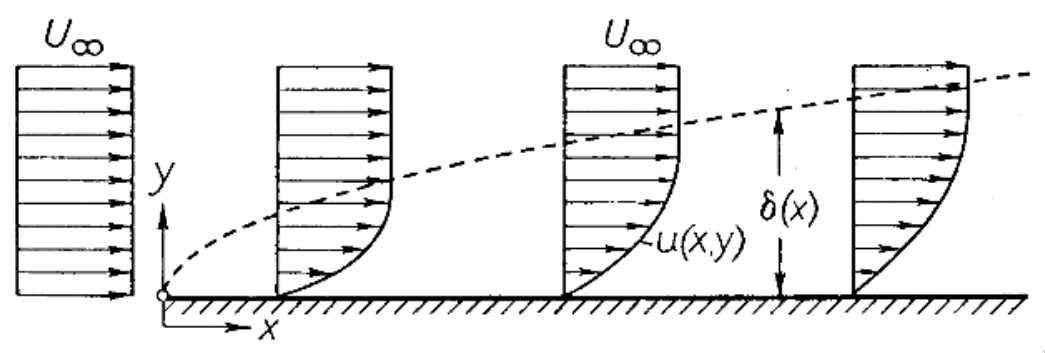
\includegraphics[width=0.5\textwidth]{boundary_layer_flat_plate}
    \caption{Laminar boundary layer of a flat plate at zero incidence
    \cite{Schlichting2018}.}
    \label{fig:boundary_layer_flat_plate}
\end{figure}

\subsubsection{Types of boundary layers}
The flow within the boundary layer can exhibit two different characteristics:
\textit{laminar} or \textit{turbulent}. In actuality, it starts as laminar at
the leading edge, then undergoes a transition to turbulence over a specific
distance, and eventually becomes fully turbulent thereafter
\cite{Schlichting2018}, this report specifically focuses on a fully turbulent
turbulence model, and as a result, the explanations of the laminar and
transitional boundary layers are not further elaborated upon.

\subsubsection{Frictional forces}
As explained earlier, the flow in the boundary layer is slowed down until it
becomes zero at the surface. This slowing down exerts a force in the flow
direction on the surface. This force, normalized by its application area, is
called \textit{shear stress} ($\tau_{w}$). To obtain a dimensionless
coefficient, which may be easily compared, the shear stress is divided by the
\textit{dynamic pressure} \cite{Schlichting2018}:

\begin{equation}
  c_{f} = \frac{\tau_{w}(x)}{\frac{1}{2}\rho U_{\infty}^{2}}
\end{equation}

\noindent Where $\rho$ is the density of the fluid and $c_{f}$ the skin friction
coefficient.


\subsection{Turbulent boundary layer}
\label{sec:turbulent_BL}
Upon closer examination of a turbulent boundary layer, one can discern two
distinct regions. The upper region constitutes a \textit{turbulent layer},
which is influenced indirectly by friction with the wall. In contrast, the
lower region is noticeably thinner compared to the overall boundary layer. This
lower region is referred to as the \textit{viscous sublayer} or \textit{viscous
wall} layer" and is directly influenced by friction. Just like the boundary
layer's broader context, there is no clear demarcation between these two
regions; instead, a smooth transition can be observed.

To analyze the cross-section of the boundary layer effectively, it is helpful
to introduce the concept of the dimensionless \textit{wall distance}, denoted
as $y^{+}$. In conjunction with this, we also consider the dimensionless
velocity, $u^{+}$. Adopting this dimensionless system facilitates the
comparison of various boundary layers from different flow conditions in a more
straightforward manner. The expression for the dimensionless velocity, $u^{+}$,
is as follows:  \cite{Schlichting2018}

\begin{equation}
  u^{+} = \frac{u}{u_{\tau}}
\end{equation}

\noindent Whereas $u$ is the flow velocity and $u_{\tau}$ the \textit{friction
velocity}. It is given by:

\begin{equation}
  u_{\tau} = \sqrt{\frac{\tau_{w}}{\rho}}
\end{equation}

\noindent As before, $\tau_{w}$ is the \textit{shear stress} and $\rho$ the
\textit{density}. The dimensionless \textit{wall distance} $y^{+}$ is given by:

\begin{equation}
  y^{+} = \frac{yu_{\tau}}{\nu}
\end{equation}

\noindent Whereas $y$ is the distance to the wall and $\nu$ is the
\textit{kinematic viscosity} of the fluid.


\subsubsection{Universal law of the wall}
Theory which describes the velocity distribution of a turbulent boundary layer
in fully developed flow\footnote{This means, the flow does not change with
increasing x.}  is know as the \textit{universal law of the wall}. It defines
the different regions as follows \cite{Schlichting2018}:

\paragraph{Viscous sublayer ($y^{+} < 5$)}
For the viscous sublayer, $u^{+}$ is given by:

\begin{equation}
  u^{+} = y^{+}
\end{equation}

\paragraph{Logarithmic overlap law ($y^{+} > 30$)}
In the fully turbulent region at the top of the boundary layer, the turbulence
stress dominates and the velocity profile varies very slowly with a logarithmic
function:

\begin{equation}
  u^{+} = \frac{1}{\kappa} ln(y^{+}) + C^{+}
  \label{eq:overlap_law}
\end{equation}

\noindent The Karman constant $\kappa$ is equal to $0.41$ and $C^{+}$ equals to
$5.0$ for smooth walls.

\paragraph{Buffer layer ($5 < y^{+} < 30$)}
The \textit{buffer layer} is located between the viscous sublayer and the
logarithmic area. It is a region where the flow transitions from one to the
other. It can not be described with such an easy equation as for the other two
regions.

If we plot the wall distance $y^{+}$ on a logarithmic scale and the velocity
$u^{+}$ on a linear scale, the different regions are obvious. Take a look at
figure \ref{fig:law_of_wall}.

\begin{figure}[H] \centering
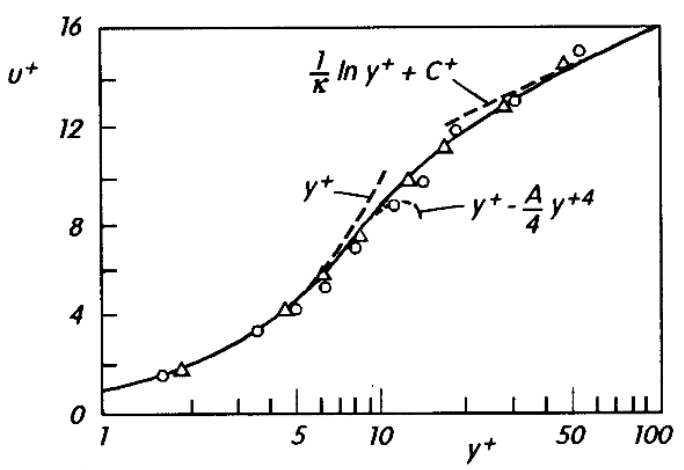
\includegraphics[width=0.45\textwidth]{law_of_wall}
    \caption{Cross section of a fully developed turbulent boundary layer
             overlayed with measurements\cite{Schlichting2018}.}
    \label{fig:law_of_wall}
\end{figure}




\section{Reynold's Averaged Navier Stokes (RANS).}
The \textit{Navier-Stokes} equations establish the connection between the
velocity ($U$), pressure ($P$), temperature ($T$), and density ($\rho$) of a
moving fluid. These equations, represented as partial differential equations,
are typically challenging to solve analytically. Consequently, numerical
methods become necessary. The physical properties are functions of four
variables: spatial coordinates (x, y, z), and time (t). To apply numerical
methods effectively, these properties must be discretized. \cite{nasaNS}

In flows with high Reynolds numbers, various eddies have significantly
different length and time scales. Properly capturing the smallest eddies,
essentially representing turbulence, would require an extremely fine mesh and
time step, rendering it impractical. To address this challenge, simplifications
are necessary: (1) considering a steady flow instead of unsteady, and (2)
accounting for turbulence in a stochastic manner. By adopting these approaches,
a single simulation (instead of one every x milliseconds) and a coarser grid
become sufficient to achieve meaningful results.


\subsubsection{Reynolds averaging}
In 1895, Osborne Reynolds introduced a solution that would later be referred to
as \textit{Reynolds Averaged Navier-Stokes}. The fundamental concept involves
dividing the velocity (along with other resolved physical properties) into two
components: \cite{leschziner2015statistical}

\begin{equation}
    U_{i} = \bar U_{i} + u_{i}^{\prime} \qquad
    P = \bar P + p^{\prime}
\end{equation}

\noindent The subscript $i$ represents all three spatial coordinates (x, y, z).
The mean velocity, denoted as $\bar U_{i}$, remains constant, while
$u_{i}^{\prime}$ represents the fluctuating component caused by turbulence,
which remains unresolved. The same notation applies to the pressure $P$.
Substituting these expressions into the incompressible Navier-Stokes equations
results in:

\begin{equation}
    \label{eq:incomp_RANS}
    \frac{\partial \rho \bar U_{i} \bar U_{j}}{\partial x_{j}} =
    \frac{\partial \bar P}{\partial x_{i}} +
    \frac{\partial}{\partial x_{j}} \nu (\frac{\partial 
    \bar U_{i}}{\partial x_{j}} +
    \frac{\partial \bar U_{j}}{\partial x_{i}}) -
    \frac{\partial}{\partial x_{j}} \rho u_{i}^{\prime} u_{j}^{\prime}
\end{equation}

\noindent The \textit{six} independent \textit{Reynolds-stresses} are
represented by $\rho u_{i}^{\prime} u_{j}^{\prime}$. It is important to note
that the fluctuating component for pressure, $p^{\prime}$, cancels out and does
not reappear. The Reynolds stresses can be denoted using tensor notation:

\begin{equation}
    \rho \bar u_{i} \bar u_{j} = \rho
    \begin{pmatrix}
        u_{1}^{\prime 2}              & u_{1}^{\prime} u_{2}^{\prime} & 
        u_{1}^{\prime} u_{3}^{\prime} \\

        u_{2}^{\prime} u_{1}^{\prime} & u_{2}^{\prime 2}              & 
        u_{2}^{\prime} u_{3}^{\prime} \\

        u_{3}^{\prime} u_{1}^{\prime} & u_{3}^{\prime} u_{2}^{\prime} & 
        u_{3}^{\prime 2}
    \end{pmatrix}
\end{equation}

\noindent Equation \ref{eq:incomp_RANS} is complemented by the Reynolds-averaged
mass-conservation equation:

\begin{equation}
    \frac{\partial \rho \bar U_{j}}{\partial x_{j}} = 0
\end{equation}


\subsubsection{Turbulence model}
To determine the unknown Reynolds stresses, a \textit{turbulence model} is
employed. Among several approaches, the two most commonly used are \textit{Eddy
viscosity} models and \textit{Reynolds stress transport} models. The SST model
belongs to the former category, and therefore, it will be elaborated on in more
detail.


\paragraph{Eddy viscosity models}
These kind of models depend on the \textit{Boussinesq-assumption} which says
that the effect of turbulence is similar to that of an increased viscosity.
Thus, it introduces the \textit{eddy viscosity} $\mu_{t}$. After some equation
mangling one may calculate the Reynolds stresses from the eddy viscosity as
follows:

\begin{equation}
    - \rho u_{i}^{\prime} u_{j}^{\prime} =
    \nu_{t} (\frac{\partial \bar U_{i}}{\partial x_{j}} +
    \frac{\partial \bar U_{j}}{\partial x_{i}}) -
    \frac{2}{3} \delta_{ij} \rho k
    \label{eq:boussinesq}
\end{equation}

\noindent Where

\begin{align*}
    \delta_{ij} = \; &0 \qquad \text{for} \qquad i \neq j \\
    &1 \qquad \text{for} \qquad i = j
\end{align*}

\noindent and $k$ is the \textit{turbulent kinetic energy}. Thus the calculation
of the six Reynolds-stresses has reduced to calculating $\nu_{t}$ and $k$.
\cite{leschziner2015statistical}




\section{Turbulence models}
The SST model is a mix between the $k$ - $\epsilon$ and $k$ - $\omega$
turbulence models. Because of that, both are explained in this section.


\subsection{$k$ - $\epsilon$ model}
This model was first introduced in 1972 and solves two transport equations
.\cite{JONES1972301} One for the turbulent kinetic energy ($k$) and one for the
dissipation rate $\epsilon$. To apply the Boussinesq-assumption, $k$ and
$\nu_t$ are needed. The first one is solved for directly and the second one is
calculated as follows:

\begin{equation}
    \nu_t = C_{\nu} \frac{\rho k^2}{\epsilon}
\end{equation}


\noindent The transport equations are as follows:
\begin{align}
    \frac{\partial (\rho k)}{\partial t} + 
    \nabla \cdot (\rho U k) &=
    \nabla \cdot \left[ 
        \left( \nu + \frac{\nu_t}{\sigma_k}\right) + \nabla k 
    \right] + P_k + P_b - \rho \epsilon + S_k \\
%
    \frac{\partial (\rho \epsilon)}{\partial t} + 
    \nabla \cdot (\rho U \epsilon) &=
    \nabla \cdot \left[ 
        \left( \nu + \frac{\nu_t}{\sigma_{\epsilon}}\right) + \nabla  \epsilon
    \right] + C_1 \frac{\epsilon}{k}(P_k + P_b) - 
    C_2 \rho \frac{\epsilon^2}{k} + S_c
\end{align}

\noindent Where $P_k$ is the production due to mean velocity shear, $P_b$ is
the production due to buoyancy and $S_k$ is a user defined source. The
remaining constants have been derived from experiments and may change.
Originally, they were defined as follows:

\begin{align*}
    C_1 &= 1.55         & C_2               &= 2.0  & C_{\nu} &= 0.09\\
    \sigma_k &= 1.0     & \sigma_{\epsilon} &= 1.3
\end{align*}

\noindent This form of the model is called the \textit{high-Reynolds-number
form}. As its name suggests, its prediction is poor near walls. This is due to
blocking effects of the wall that lower the dissipation. The original authors
proposed an extension that is better suited. This is called
\textit{low-Reynolds-number form}. The model is modified as follows:

\begin{align}
    \nu_t = \textcolor{red}{f_{\nu}} C_{\nu} \frac{\rho k^2}{\epsilon},  \qquad
%
    ... + C_1 \frac{\epsilon}{k}(\textcolor{red}{f_1} P_k + P_b) 
    - \textcolor{red}{f_2} C_2 \rho \frac{\epsilon^2}{k} + ..
\end{align}

\noindent Where the modifications in red are damping functions that are defined
as follows:

\begin{align}
    f_1 &= 1 \\
    f_2 &= 1 - 0.3 exp(-Re_T^2) \\
    f_{\nu} &= exp \left( \frac{-3.4}{(1 + (Re_T/50))^2}\right) \\
\end{align}

\noindent Where $Re_T$ is the turbulent Reynolds number which is:

\begin{equation}
    Re_T = \frac{\rho k^2}{\nu \epsilon} 
\end{equation}

\noindent The damping function $f_{\nu}$ tends to be 1 far from the wall
because $Re_T$ tends to be high there. Close to the wall, $f_{\nu}$, where
$Re_T$ is low, goes towards 0 and thus the effects of the eddy viscosity
vanish. The original authors did not see an improvement for $f_1$ and therefore
left it at 1. The function $f_2$ is applied to the dissipation of $\epsilon$
and consequently lowers it near the wall it.


\paragraph{Conclusion}
This model works well for prediction flows outside of boundary layers. Although
it has the capacity to predict the flow near the wall, inside the boundary
layer, it does so poorly. If there are \textbf{adverse pressure gradients}
and/or \textbf{shocks} present, the prediction inside the boundary layer is
even worse. \cite{cfd101_k-epsilon}



\subsection{$k$ - $\omega$ model}
Because of the shortcomings mentioned in the section before, a better
turbulence model was needed for aerodynamics and turbumachinery.






\subsection{$k$ - $\omega$ SST model}




\section{Algorithmic Differentiation and the adjoint method}
\subsection{Overview}
briefly explain AD and adjoint. Reference to adjoint report. Also mention  


\subsection{Verification}
How those things can be validated 
\subsubsection{Finite Differences}
\subsubsection{Complex Step}
\subsubsection{Dot Product Test}




\section{Grid Convergence}
When discretizing a partial differential equation and solving it numerically,
an error is introduced. It may be decreased through a finer mesh or a higher
order method. To demonstrate that the method approaches the exact solution,
finder and finer grids are used. This process is called a \textit{grid
refinement study} or \textit{mesh convergence}. For a given grid, the grid
spacing is:

\begin{equation}
  h = N^{-1/d}
\end{equation}

\noindent Where $N$ is the number of cells and $d$ is the dimension of the
problem.
For ADflow, the expected rate of convergence is $p=2$. But in reality, this
might not be the case. For three grids, the actual rate may be calculated as
follows:

\begin{equation}
  \hat p = ln(\frac{f_{L2} - f_{L1}}{f_{L1} - f_{L0}}) / ln(r)
  \label{eq:conv_rate}
\end{equation}

\noindent Where $f$ is the function of interest (e.g. $c_{d}$) and the subscript
tells the grid used. $L0$ is the finest grid and $L2$ the coarsest. The
parameter $r$ is the grid refinement ratio .\cite{grid_refinement}
